% begin module newtons-method-def
\begin{frame}
\begin{columns}[c]
\column{.4\textwidth}
Goal: find a root $r$ of $f(x)$.
\psset{xunit=0.9cm, yunit=0.9cm}
\begin{pspicture}(-0.5,-0.5)(4.6,4.1)
\psframe*[linecolor=white](-0.5,-0.5)(4.6,4.1)
\psaxes[ticks=none, labels=none]{<->}(0,0)(-0.5,-0.5)(4.5,4)\tiny
\fcLabels{4.5}{4}
%Function formula: (1/2 (x))^{2}-3/10
\rput[r](2.8,2){$y=f(x)$}
\psplot[linecolor=red, plotpoints=1000]{0}{4}{-0.3 x 0.5 mul 2 exp add }
\fcXTick{1.095445115}
\rput[b](1.095445115, 0.2){$r$}

\uncover<2->{\fcLabelOnXaxis{4}{\alertNoH{2}{$x_1$}}} %x_1:=4; f{}x_1:=3.7;
\uncover<3-5,10-20>{
\psline[linestyle=dashed](4,0)(4,3.7)
\fcFullDot{4}{3.7}
%Function formula: -43/10+2 (x)
\psplot[linecolor=\fcColorTangent, plotpoints=1000]{2}{4}{x 2 mul -4.3 add }
}

\uncover<4->{\fcLabelOnXaxis{2.15}{\alertNoH{4,20}{$x_2$}}} %x_2:=43/20; f{}x_2:=0.855625;

\uncover<6-7,21-32>{
\psline[linestyle=dashed](2.15,0)(2.15,0.855625)
\fcFullDot{2.15}{0.855625}
%Function formula: -2329/1600+43/40 (x)
\psplot[linecolor=\fcColorTangent, plotpoints=1000]{1.1}{4}{x 1.075 mul -1.45562 add }
}

\uncover<7->{\fcLabelOnXaxis{1.354069767}{\alertNoH{7,32}{$x_3$}}} %x_3:=1354069767/1000000000; f{}x_3:=0.158376;
\uncover<8>{
\psline[linestyle=dashed](1.354069767,0)(1.354069767,0.158376)
\fcFullDot{1.354069767}{0.158376}
%Function formula: -3033504933903434289/4000000000000000000+1354069767/2000000000 (x)
\psplot[linecolor=\fcColorTangent, plotpoints=1000]{0.7}{4}{x 0.677035 mul -0.758376 add }
}
\uncover<8->{
\fcLabelOnXaxis{1.120143514}{\alertNoH{8}{$x_4$}}
} %x_4:=1011168311301144763/902713178000000000

\end{pspicture}

%\ \only<handout:0| -2>{%
%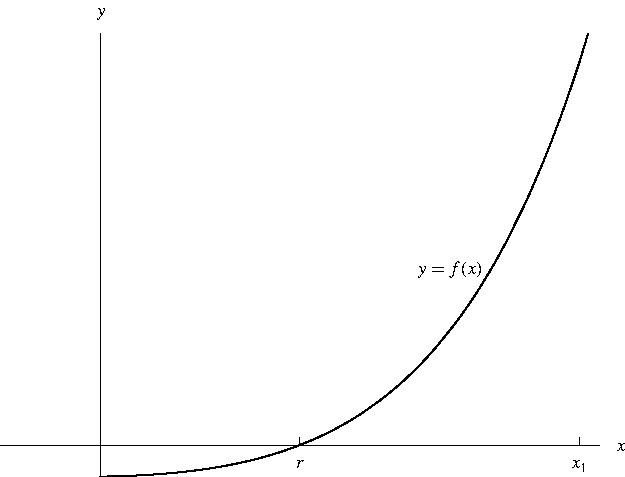
\includegraphics[height=4cm]{newtons-method/pictures/04-08-newtona.pdf}%
%}%
%\only<handout:0| 3-5,10-20>{%
%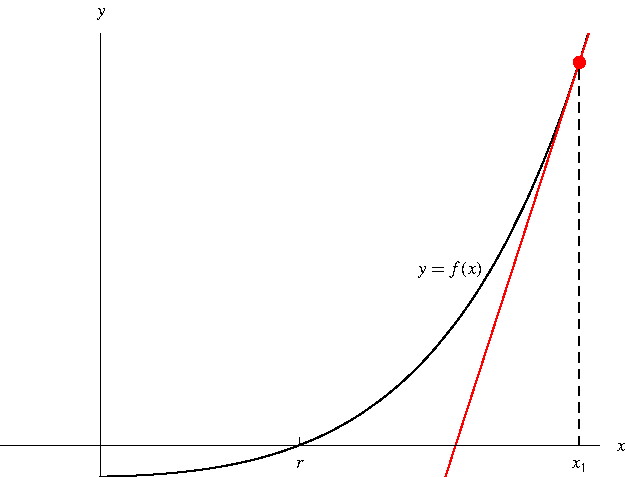
\includegraphics[height=4cm]{newtons-method/pictures/04-08-newtonb.pdf}%
%}%
%\only<handout:0| 6-7,22-22>{%
%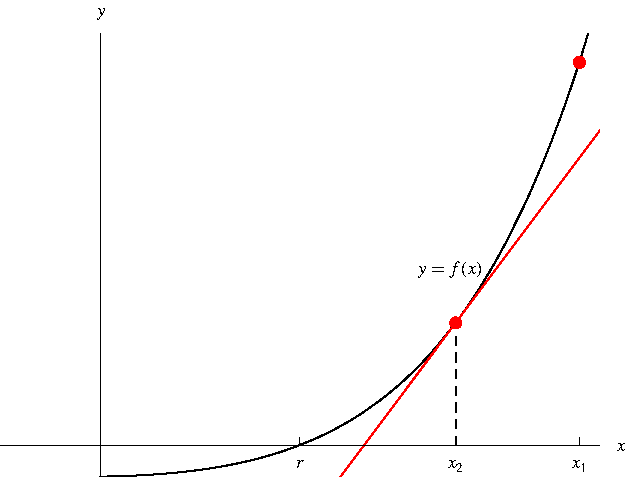
\includegraphics[height=4cm]{newtons-method/pictures/04-08-newtonc.pdf}%
%}%
%\only<handout:0| 8>{%
%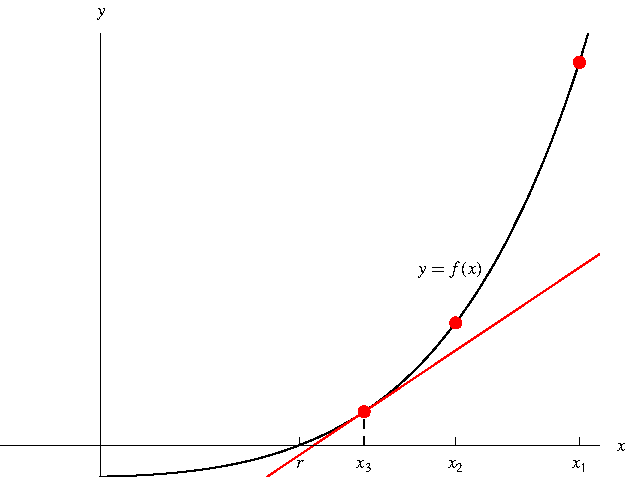
\includegraphics[height=4cm]{newtons-method/pictures/04-08-newtond.pdf}%
%}%
%\only<9,23->{%
%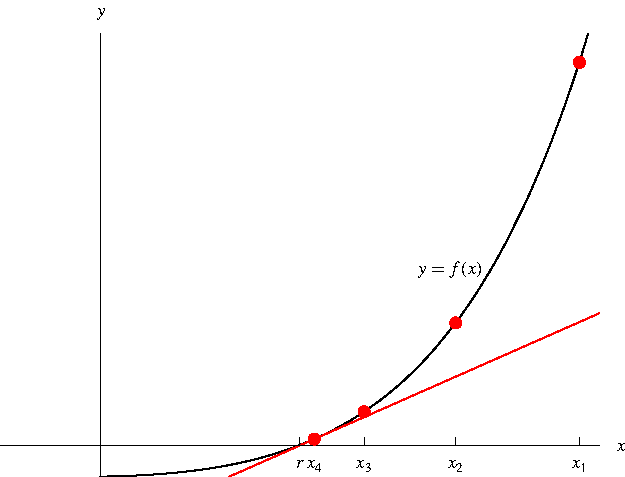
\includegraphics[height=4cm]{newtons-method/pictures/04-08-newtone.pdf}%
%}%

\column{.6\textwidth}

\begin{itemize}
\item<2->  Pick a number $x_1$.
\item<3-| alert@10-13>  Find the tangent to $f$ at $(x_1, f(x_1))$.
\item<4-| alert@14-20>  Call the $x$-intercept of this line $x_2$.
\item<5->\alertNoH{21}{Repeat the process using $x_2$.} 
\item<6-| alert@22-25>  Find the tangent to $f$ at $(x_2, f(x_2))$.
\item<7->  \alertNoH{26-32}{Call the $x$-intercept of this line $x_3$}, \uncover<8->{ \alertNoH{8,33}{and so on.}}
\end{itemize}
\end{columns}
\vskip -0.1cm
\begin{columns}[c]
\column{.35\textwidth}
\[
\begin{array}{rcl}
\uncover<20->{\alertNoH{20}{x_2} &\alertNoH{20}{=}&\displaystyle  \alertNoH{20}{ x_1 - \frac{f( x_1)}{f'(x_1)}}} \\%
\uncover<32->{\alertNoH{32}{x_3} &\alertNoH{32}{=}&\displaystyle  \alertNoH{32}{ x_2 - \frac{f (x_2)}{f'(x_2)}}}\\%
\uncover<33->{&\vdots&} \\
\uncover<34->{ \alertNoH{34}{x_{n+1}} &\alertNoH{34}{=} &\displaystyle  \alertNoH{34}{x_n - \frac{ f(x_n)}{ f'(x_n)}}}
\end{array}
\]
\column{.65\textwidth}
\abovedisplayskip=0pt
\belowdisplayskip=-15pt
\uncover<10-20, 22-32,34->{
\[
\begin{array}{r@{}c@{}l}
\displaystyle \text{Equation:}\quad
\alertNoH{14,26}{ y} -  \onlyNoH{-20}{\fcAnswerUncover{10}{13}{f(x_1)}}
\onlyNoH{22-32}{\fcAnswerUncover{22}{25}{f(x_2)}}
\only<34->{f(x_n)}
& \alertNoH{0}{=}& \displaystyle
\onlyNoH{-20}{\fcAnswer{11}{f'(x_1)}}
\onlyNoH{22-32}{\fcAnswer{23}{f'(x_2)}}
\only<34->{f'(x_n)}
(\alertNoH{14,26}{x}-
\onlyNoH{-20}{\fcAnswerUncover{10}{13}{x_1}}
\onlyNoH{22-32}{\fcAnswerUncover{22}{25}{x_2}}
\only<34->{x_n}
)
\\
\displaystyle \uncover<14-20,26-32,34->{\text{$x$-intercept:}\quad
\alertNoH{ 14,26}{0} - 
\onlyNoH{-20}{f(x_1)}
\onlyNoH{22-32}{f(x_2)}
\only<34->{f(x_n)}
& \alertNoH{0}{=} & \displaystyle
\onlyNoH{-20}{\alertNoH{15,16}{f'(x_1)}}
\onlyNoH{22-32}{\alertNoH{27,28}{f'(x_2)}}
\only<34->{f'(x_n)}
(
\onlyNoH{-20}{\alertNoH{14,15}{x_2}}
\onlyNoH{22-32}{\alertNoH{26,27}{x_3}}
\only<34->{x_{n+1}}
\onlyNoH{-20}{\alertNoH{16}{-x_1}}
\onlyNoH{22-32}{\alertNoH{28}{-x_2}}
\only<34->{-x_{n}}
)}\\
\displaystyle \uncover<15-20, 27->{
\onlyNoH{-20}{\alertNoH{16,17}{f'(x_1)x_1}}
\onlyNoH{22-32}{\alertNoH{28,29}{f'(x_2)x_2}}
\only<34->{f'(x_n)x_n}
\onlyNoH{-20}{\alertNoH{17}{-f(x_1)}}
\onlyNoH{22-32}{\alertNoH{29}{-f(x_2)}}
\only<34->{-f(x_n)}
& \alertNoH{0}{=} & \displaystyle
\onlyNoH{-20}{\alertNoH{15}{\alertNoH{18}{f'(x_1)}x_2}}
\onlyNoH{22-32}{\alertNoH{27}{\alertNoH{30}{f'(x_2)}x_3}}
\only<34->{f'(x_n)x_{n+1}}
}\\
\displaystyle \uncover<17-20, 29->{
\onlyNoH{-20}{x_2}
\onlyNoH{22-32}{x_3}
\only<34->{x_{n+1}}
& = &\displaystyle
\onlyNoH{-20}{\frac{\alertNoH{17}{\alertNoH{19}{f'(x_1)x_1}-f(x_1)}}{\alertNoH{18,19}{f'(x_1)}}}
\onlyNoH{22-32}{\frac{\alertNoH{29}{\alertNoH{31}{f'(x_2)x_2}-f(x_2)}}{\alertNoH{30,31}{f'(x_2)}}}
\only<34->{\frac{f'(x_n)x_n-f(x_n)}{f'(x_n)}}
}\\
\displaystyle\uncover<19-20, 31->{
\onlyNoH{-20}{ \alertNoH{20}{x_2}}
\onlyNoH{22-32}{ \alertNoH{32}{x_3}}
\only<34->{\alertNoH{34}{x_{n+1}}}
&\alertNoH{20,32,34}{=}&\displaystyle \onlyNoH{-20}{\alertNoH{20}{\alertNoH{19}{x_1}-\frac{ f(x_1)}{f'(x_1)} }}
\onlyNoH{22-32}{\alertNoH{32}{\alertNoH{31}{x_2}-\frac{ f(x_2)}{f'(x_2)} }}
\only<34->{\alertNoH{34}{x_n-\frac{ f(x_n)}{f'(x_n)} }}
}
\end{array}
\]
}
\end{columns}
\end{frame}
% end module newtons-method-def
